\documentclass{beamer}
\usetheme{Rochester}
\usepackage{tcolorbox}
\tcbuselibrary{listings}
\usepackage{inconsolata}

\geometry{paperwidth = 4.75in, paperheight = 4.75in}

% Custom U of C color palette
\definecolor{ucMaroon}{RGB}{128,0,0}
\definecolor{ucDarkGray}{RGB}{118,118,118}
\definecolor{ucLightGray}{RGB}{214,214,206}

\setbeamercolor{block title}{fg=white,bg=ucMaroon}
\setbeamercolor{block title alerted}{use=alerted text,fg=white,bg=alerted text.fg}
\setbeamercolor{block title example}{use=example text,fg=white,bg=example text.fg}
\setbeamercolor{block body}{parent=normal text,use=block title,bg=ucLightGray}
\setbeamercolor{block body alerted}{parent=normal text,use=block title alerted,bg=block title alerted.bg}
\setbeamercolor{block body example}{parent=normal text,use=block title example,bg=block title example.bg}

\setbeamercolor{palette primary}{fg=white,bg=ucMaroon}
\setbeamercolor{palette secondary}{fg=white,bg=ucLightGray}
\setbeamercolor{palette tertiary}{fg=white,bg=ucDarkGray}
\setbeamercolor{palette quaternary}{fg=white,bg=black}

\setbeamercolor{sidebar}{bg=ucMaroon}

\setbeamercolor{palette sidebar primary}{fg=ucMaroon}
\setbeamercolor{palette sidebar secondary}{fg=white}
\setbeamercolor{palette sidebar tertiary}{fg=ucMaroon}
\setbeamercolor{palette sidebar quaternary}{fg=white}

\setbeamercolor{titlelike}{parent=palette primary}
\setbeamercolor{itemize item}{fg=ucMaroon}

% Code block formatting. Fragile frames needed for these to work.
\newtcblisting{gitCommand}{
  colframe=black,
  colback=ucLightGray,
  boxrule=1pt,
  arc=2pt,
  left=6pt,
  right=6pt,
  top=6pt,
  bottom=6pt,
  before=\vspace{6pt},
  boxsep=0pt,
  listing only,
  hbox
}


\title{Intermediate Git}
\subtitle{Day 2: Ignoring Files and Fixing Mistakes}
\author{Raman A.~Shah}
\date{}

\begin{document}

%% Title
\begin{frame}[plain]
  \titlepage
  \footnotesize{Copyright (c) 2015 by Raman A.~Shah.\\
  \href{https://creativecommons.org/licenses/by-nc-sa/3.0/legalcode}
       {Creative Commons BY-NC-SA 3.0 Unported}.\\
   \href{https://github.com/ramanshah/intermediate\_git}
        {https://github.com/ramanshah/intermediate\_git}}
\end{frame}

%% Use .gitignore for...
\begin{frame}{Use \texttt{.gitignore} for \ldots}
  \hangindent=26pt \huge {
  \ldots secrets.
  }
\end{frame}

\begin{frame}{Use \texttt{.gitignore} for \ldots}
  \hangindent=26pt \huge {
  \ldots local configuration.
  }
\end{frame}

\begin{frame}{Use \texttt{.gitignore} for \ldots}
  \hangindent=26pt \huge {
  \ldots large unnecessary files.
  }
\end{frame}

\begin{frame}{Use \texttt{.gitignore} for \ldots}
  \hangindent=26pt \huge {
  \ldots junk from your operating system and development environment.
  }
\end{frame}

%% Glob patterns
\begin{frame}[fragile]{``Glob patterns''}
  Ignore any file ending with \texttt{.txt}:

  \begin{gitCommand}*.txt\end{gitCommand}

  But don't ignore \texttt{IMPORTANT.txt}:

  \begin{gitCommand}!IMPORTANT.txt\end{gitCommand}

  Ignore \texttt{temp0.out}, \ldots, \texttt{temp9.out}, but not
  \texttt{tempa.out}:

  \begin{gitCommand}temp[0-9].out\end{gitCommand}

  Ignore \texttt{temp0.out}, \ldots, \texttt{temp9.out}, and also
  \texttt{tempa.out} (but not \texttt{temp\_a.out}):

  \begin{gitCommand}temp?.out\end{gitCommand}
\end{frame}

\begin{frame}[fragile]{``Glob patterns,'' continued}
  Ignore file \texttt{JUNK.tmp} anywhere in the repo:

  \begin{gitCommand}JUNK.tmp\end{gitCommand}

  Ignore file \texttt{JUNK.tmp} in the root directory, but don't ignore
  \texttt{subdir/JUNK.tmp}:

  \begin{gitCommand}/JUNK.tmp\end{gitCommand}

  Ignore all files in the subdirectory \texttt{subdir}:

  \begin{gitCommand}subdir/\end{gitCommand}

  Ignore \texttt{log/foo.log} but not \texttt{foo.log} in the root directory:

  \begin{gitCommand}log/*.log\end{gitCommand}
\end{frame}

%% Initializing a Git repository
\begin{frame}[fragile]{Initializing a Git repository}
  Download a compressed example of a messy project not under version control:

  \begin{gitCommand}
git clone https://github.com/\
ramanshah/intermediate_git.git
  \end{gitCommand}

  Pull it out of the course repo and decompress it into a directory:

  \begin{gitCommand}
cp ./intermediate_git/day2/sample.tgz .
tar xzvf sample.tgz
cd sample
  \end{gitCommand}
\end{frame}

\begin{frame}[fragile]{Initializing a Git repository}
  From the directory that you're hoping to turn into a Git repository:

  \begin{gitCommand}git init\end{gitCommand}

  Survey the candidates to put under version control:

  \begin{gitCommand}git status\end{gitCommand}

  Survey the files within a subdirectory:

  \begin{gitCommand}git ls-files --others \
  --exclude-standard [subdir]
  \end{gitCommand}
\end{frame}

\begin{frame}[fragile]{Staging your changes}
  To stage a modified file for the next commit:

  \begin{gitCommand}git add [path]\end{gitCommand}

  To unstage a staged file:

  \begin{gitCommand}git reset HEAD [path]\end{gitCommand}

  When ready to commit:

  \begin{gitCommand}git commit\end{gitCommand}

  To write a commit message inline:

  \begin{gitCommand}git commit -m [message]\end{gitCommand}

\end{frame}

\begin{frame}{Examining the staging area}
  \begin{figure}
    \includegraphics[scale=0.32]{diffs.pdf}
  \end{figure}
\end{frame}

\begin{frame}{Manipulating files}
  \begin{figure}
    \includegraphics[scale=0.32]{manipulations.pdf}
  \end{figure}
\end{frame}

\begin{frame}[fragile]{Removing files}
  To stage a file for deletion (and simultaneously delete it from the
  working tree):

  \begin{gitCommand}git rm [path]\end{gitCommand}

  Git will complain if there are local or staged changes. To force removal:

  \begin{gitCommand}git rm -f [path]\end{gitCommand}

  To stage the file for deletion only from the Git history, leaving the working directory alone:

  \begin{gitCommand}git rm --cached [path]\end{gitCommand}
\end{frame}

\begin{frame}[fragile]{Moving files}
  Because of content addressability, this:

  \begin{gitCommand}git mv [old path] [new path]\end{gitCommand}

  is the same as this:

  \begin{gitCommand}
mv [old path] [new path]
git rm [old path]
git add [new path]
  \end{gitCommand}

\end{frame}

%% Fixing common mistakes
\begin{frame}{Fixing common mistakes}
  \begin{figure}
    \includegraphics[scale=0.35]{climbing-756669_640.jpg}
    \\ Git gives you anchors!
  \end{figure}
\end{frame}

%% I screwed everything up but didn't commit. How do I return to my most recent commit?
\begin{frame}[fragile]{Uncommitted mistake \#1}

  \color{ucMaroon}{I screwed everything up but didn't commit. How do I return
  to my most recent commit?}

  \qquad

  \begin{gitCommand}git reset --hard HEAD\end{gitCommand}
\end{frame}

%% Scopes of git reset
\begin{frame}{Scopes of git reset}
  \begin{figure}
    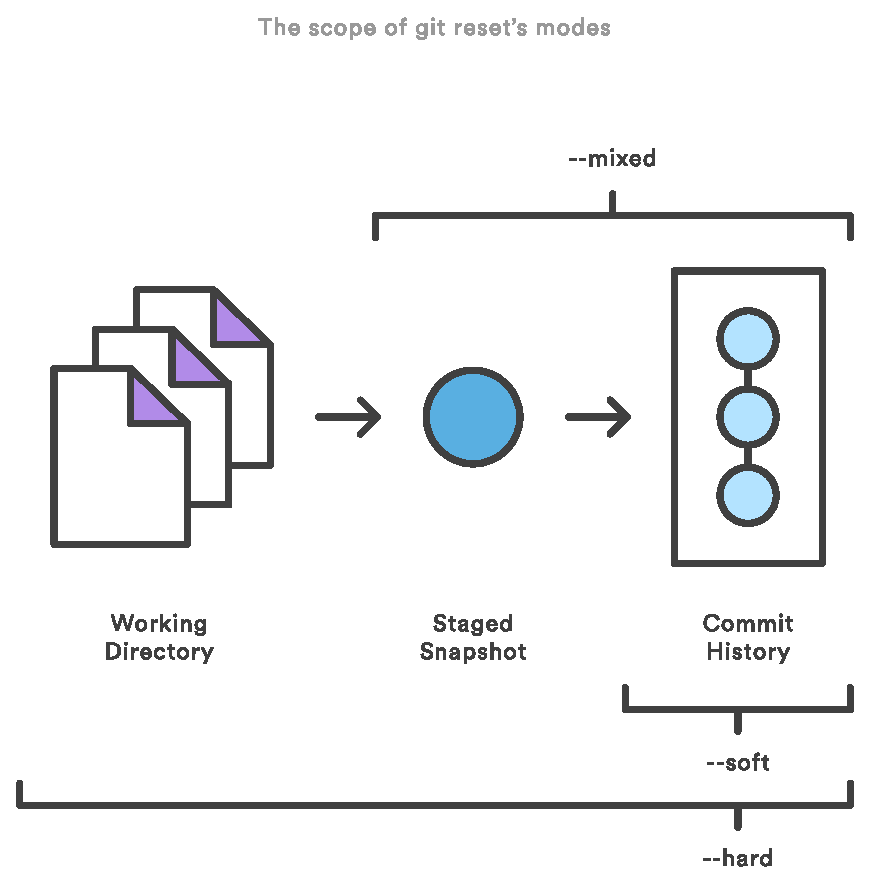
\includegraphics[scale=0.4]{reset_scopes.eps}
    \\ \texttt{--mixed} is the default.
  \end{figure}
  \footnotesize{Atlassian,
    \emph{Reset, Checkout, and Revert}.\\
    \href{http://creativecommons.org/licenses/by/2.5/au/legalcode}{CC-BY Australia}.
    \href{https://www.atlassian.com/git/tutorials/}
    {https://www.atlassian.com/git/tutorials/}}

\end{frame}

%% I modified one file incorrectly but didn't commit. Can I restore just that one file?
\begin{frame}[fragile]{Uncommitted mistake \#2}

  \color{ucMaroon}{I modified one file incorrectly but didn't commit. Can I
  restore just that one file?}

  \qquad

  \begin{gitCommand}git checkout HEAD [path]\end{gitCommand}
\end{frame}

%% I forgot to ignore something, and now it has changed and is chasing me around.
\begin{frame}[fragile]{Committed mistake \#1}

  \color{ucMaroon}{I forgot to ignore something, and now it has changed and is
  chasing me around.}

  \qquad

  \color{black}{First, mark it for deletion in the staging area only:}

  \begin{gitCommand}git rm --cached [path]\end{gitCommand}

  Then commit the deletion:

  \begin{gitCommand}git commit\end{gitCommand}

  Then fix your \texttt{.gitignore} and commit the changes to \texttt{.gitignore}.

\end{frame}

%% My most recent commit is half-baked. Can I bake it better?
\begin{frame}[fragile]{Committed mistake \#2}

  \color{ucMaroon}{My most recent commit is half-baked. Can I bake it better?}

  \qquad

  \color{black}{Stage your corrections:}

  \begin{gitCommand}git add [path]\end{gitCommand}

  Then commit with a fresh message:

  \begin{gitCommand}git commit --amend\end{gitCommand}
\end{frame}

%% Commit message style guide
\begin{frame}{Commit message style guide}
  \begin{itemize}
    \item First line: $ \le 50 $ columns, imperative mood.
    \item Second line: blank.
    \item Subsequently: paragraph form, 72 columns, blank line between
          paragraphs.
  \end{itemize}

  \begin{figure}
    \includegraphics[scale=0.35]{pope_commit_message.png}
  \end{figure}
  \footnotesize{Tim Pope,
    \href{http://tbaggery.com/2008/04/19/a-note-about-git-commit-messages.html}
         {\emph{A Note About Git Commit Messages}}}
\end{frame}

%% I wish the last commit never happened. Can we throw it away?
\begin{frame}[fragile]{Committed mistake \#3}
  \color{ucMaroon}{I wish the last commit never happened. Can I throw it away?}

  \begin{gitCommand}git reset --hard HEAD~1\end{gitCommand}
\end{frame}

%% I wish the last n commits never happened, but I want to keep the
%% current stuff in the working tree.
\begin{frame}[fragile]{Committed mistake \#4}
  \color{ucMaroon}{I wish the last $ n $ commits never happened, but I want
  to keep the current stuff in the working tree.}

  \begin{gitCommand}git reset HEAD~n\end{gitCommand}
\end{frame}

%% The Golden Rule of Git
\begin{frame}{The Golden Rule of Git}
  \huge {
  Never modify history that someone else has seen.
  }
\end{frame}

%% git revert
\begin{frame}[fragile]{In public: git revert}
  Instead of deleting history with \texttt{git reset}, make \emph{new}
  commits that reverse the damage done by a specified commit:

  \begin{gitCommand}git revert HEAD~1\end{gitCommand}
\end{frame}
\end{document}
